\documentclass[tikz,dvipsnames]{standalone}
\usetikzlibrary{decorations.pathmorphing, decorations.pathreplacing, decorations.shapes}
\usetikzlibrary{shapes.symbols}
\usepackage[OT1]{fontenc}
\renewcommand*\familydefault{\sfdefault}


\begin{document}

    
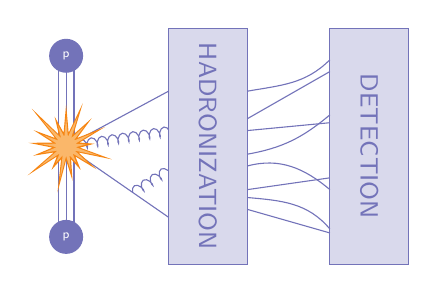
\begin{tikzpicture}

    \node (a) at (0,2.25) {};
    \node (b) at (0,4.75) {};
    \node (c) at (0.1,2.15) {};
    \node (d) at (0.1,4.75) {};
    \node (e) at (-0.1,2.15) {};
    \node (f) at (-0.1,4.75) {};

    \draw[color=NavyBlue!55] (a)--(b);
    \draw[color=NavyBlue!55] (c)--(d);
    \draw[color=NavyBlue!55] (e)--(f);

    \node[circle, fill,color=NavyBlue!55,scale=0.9] at (0,2.35) {\tiny\textcolor{White}{p}};
    \node[circle, fill,color=NavyBlue!55,scale=0.9] at (0,4.65) {\tiny\textcolor{White}{p}};

    \draw[color=NavyBlue!55] (0,3.5)--(1.3,4.2);
    \draw[color=NavyBlue!55] (0,3.5)--(1.3,2.6) node[pos=0.65] (g) {};

    \draw[decorate,decoration={coil,segment length=3.8pt,amplitude=0.6mm},color=NavyBlue!55] (0,3.5)--(1.35,3.7) ;
    \draw[decorate,decoration={coil,segment length=3.8pt,amplitude=0.6mm},color=NavyBlue!55] (g.center)--(1.3,3.2);

    \node[starburst, minimum width=1.35cm, minimum height=1.35cm,fill,color=BurntOrange] at (0,3.5) {};
    \node[starburst, minimum width=1.35cm, minimum height=1.35cm,fill,color=BurntOrange!55,scale=0.7] at (0,3.5) {};
    \filldraw[fill=NavyBlue!15,draw=NavyBlue!55] (1.3,2) rectangle ++(1,3);

    \node[rotate=-90,color=NavyBlue!55] at (1.8,3.5) {\small{HADRONIZATION}};

    \filldraw[draw=NavyBlue!55,fill=NavyBlue!15] (3.35,2) rectangle ++(1,3);

    \node[rotate=-90,color=NavyBlue!55] at (3.85,3.5) {\small{DETECTION}};

    \draw[color=NavyBlue!55] (2.3,3.7) -- (3.35,3.8);
    \draw[color=NavyBlue!55] (2.3,2.95) -- (3.35,3.1);
    \draw[color=NavyBlue!55] (2.3,2.7) -- (3.35,2.4);
    \draw[color=NavyBlue!55] (2.3,3.85) -- (3.35,4.45);


    \draw[color=NavyBlue!55] (2.3,2.85) to[out=-5,in=130] (3.35,2.45);
    \draw[color=NavyBlue!55] (2.3,3.25) to[out=15,in=140] (3.35,2.95);
    \draw[color=NavyBlue!55] (2.3,3.4) to[out=10,in=-140] (3.35,3.9);
    \draw[color=NavyBlue!55] (2.3,4.2) to[out=10,in=-135] (3.35,4.6);

\end{tikzpicture}


\end{document}